\section{Технология сравнительного эксперимента}
\begin{algorithm}[H]
\small\setstretch{1.05}
\caption{Воспроизводимое сравнение тестовых раннеров}
\begin{algorithmic}[1]
\Require Наборы $\mathcal D$, раннеры $F$, повторы $r_{\max}$, $q$, seed
\State Проверить входные наборы общим модулем утверждений
\State Сохранить версии, конфигурации и хеши файлов
\ForAll{$(D,f)\in\mathcal D\times F$}
  \State Выполнить один исключаемый прогревочный запуск
  \State При ошибке остановить эксперимент
\EndFor
\For{$r=1,\ldots,r_{\max}$}
  \State $B\gets$ перестановка $\mathcal D\times F$ с заданным seed
  \ForAll{$(D,f)\in B$}
    \State Создать процесс раннера с входом $D$ и повтором $q$
    \While{процесс работает}
      \State Обнаружить потомков, записать CPU и сумму RSS
      \State Проверить тайм-аут; выдержать паузу между отсчётами
    \EndWhile
    \State Сохранить время, код выхода, журнал и качество отсчётов
  \EndFor
\EndFor
\State Для успешных наблюдений вычислить медианы и квартили
\State При неуспешных запусках завершить команду с ошибкой
\end{algorithmic}
\end{algorithm}

Перестановка строится блоками: каждая комбинация набора и раннера появляется ровно один раз в каждом раунде. Это уменьшает систематическое преимущество инструмента, который всегда запускался первым или последним. Seed фиксирует порядок, но не делает продолжительность детерминированной: планировщик и фоновые процессы продолжают влиять на результаты.

Каждый замер создаёт новый процесс. Прогрев относится к файлам и кэшам среды, но не сохраняет JIT-состояние между процессами. Внутри одного запуска десять повторений нагрузки позволяют функции исполняться многократно. Поэтому корректное название сценария -- повторный пакетный запуск с новым процессом и сохранением кэшей ОС. Термин «полностью холодный запуск» к нему не применяется.

\section{Разработанное программное обеспечение}
Стенд разделяет измеряемую программу и наблюдатель. JavaScript-модули читают вход, вычисляют палиндромы и выполняют утверждения. Python запускает раннеры как дочерние процессы и наблюдает ресурсы извне. Его собственная память не суммируется с памятью измеряемого дерева, хотя вычислительная работа наблюдателя способна косвенно влиять на планирование.

\begin{table}[H]\centering\small
\caption{Основные компоненты приложения}
\begin{tabularx}{\linewidth}{lX}
\toprule
Файл & Назначение\\\midrule
\code{src/cli.js} & Консольный ввод строки, JSON и стандартного потока\\
\code{src/manacher.js} & Чистая функция и безопасное преобразование строки\\
\code{src/data-loader.js} & Разбор и валидация JSON/CSV\\
\code{src/run-suite.js} & Общие утверждения, внутренние повторы\\
\code{src/benchmark.js} & Сравнение с отдельным эталонным выходом\\
\code{src/demo.js} & Авторский пример и печать радиусов\\
\code{tests/*/manacher.test.js} & Тонкие адаптеры трёх раннеров\\
\code{tests/shared.cjs} & Общие функциональные и консольные проверки\\
\code{generate.py} & Масштабируемые входы с независимыми ожиданиями\\
\code{benchmark.py} & Измерение, журналы, сводка и метаданные\\\bottomrule
\end{tabularx}
\end{table}

Общий модуль выполняет строгое сравнение максимального палиндрома и числа вхождений для каждой строки. Положительный результат одного лишь запуска раннера недостаточен: ошибка в любом ожидании приводит к исключению. Адаптеры вызывают один и тот же модуль, что устраняет различия в логике тестов.

Результаты предыдущих внутренних повторов не накапливаются: сохраняется только последний проход. Иначе потребление памяти отражало бы искусственный массив из копий ответов, а не рабочую память алгоритма и раннера. Код снабжён комментариями в местах, существенных для корректности и методики.

Проект не требует сборщика приложения или компиляции TypeScript. После установки зависимостей исходники JavaScript сразу готовы к запуску. Версии JavaScript-пакетов закреплены в \code{package.json} и транзитивно в \code{package-lock.json}. Реальный файл \code{requirements.txt} фиксирует зависимость наблюдателя от psutil.

\section{Консольный интерфейс приложения}
Приложение решает самостоятельную пользовательскую задачу: находит самый длинный палиндром и число всех палиндромных вхождений. Для обычного расчёта пользователь не должен заранее знать ответ. Поэтому интерфейс расчёта отделён от тестового загрузчика с эталонными ожиданиями.

Основной запуск из каталога \code{benchmark_app}:
\begin{lstlisting}
npm start -- --text "abba"
npm start -- --file data/input-example.json
node src/cli.js --json '{"input":"abba"}'
node src/cli.js --text "abba" --output-json --radii
\end{lstlisting}
Последняя команда выводит машиночитаемый JSON с результатами. Имена ключей \code{longest}, \code{length}, \code{count} и \code{radii} сохраняются стабильными для автоматической обработки. Текстовые сообщения и названия тестов написаны на русском. Служебный вывод самих сторонних раннеров, например PASS и Tests, формируется их библиотеками.

Для строки \code{abba} консоль показывает:
\begin{Verbatim}[fontsize=\small,frame=single]
Самый длинный палиндром: "abba"
Длина: 4
Число палиндромных вхождений: 6
\end{Verbatim}
Одинаковые буквы на разных позициях считаются разными вхождениями. Параметр \code{--radii} добавляет массив радиусов и помогает сопоставить запуск с пошаговой таблицей алгоритма.

Если запустить \code{npm start} в интерактивном терминале без аргументов, программа запросит строку. Для пустого ввода достаточно нажать Enter. Параметр \code{--text} позволяет передать строку, начинающуюся с двух дефисов, не принимая её за параметр. Справка доступна через \code{--help}.

Пользовательский JSON допускает строку, объект с полем \code{input}, массив строк или объектов, а также объект с массивом \code{cases}. Например:
\begin{Verbatim}[fontsize=\small,frame=single]
{"cases": [
  {"name": "Чётный палиндром", "input": "abba"},
  {"name": "Русская строка", "input": "топот"},
  {"name": "Пустая строка", "input": ""}
]}
\end{Verbatim}
Поля ожидаемого ответа не требуются. При передаче тестового файла приложению они не участвуют в расчёте: проверку ожиданий выполняют команды тестов и \code{verify}. Неправильный тип \code{input}, пустой пакет, повреждённый JSON, отсутствующий файл или конфликт источников ввода дают русское сообщение в стандартном потоке ошибок и код завершения 1.

Для автоматизации предусмотрен \code{--stdin}. Совместно с \code{--json} он читает весь поток как JSON, иначе как исходную строку. Пробелы и завершающие переводы строки сохраняются. Это важно при конвейерном вводе: перевод строки, добавленный оболочкой, является частью задачи. Входной UTF-8 BOM удаляется только при разборе JSON.

Интерфейс обрабатывает Unicode по кодовым точкам без нормализации и без изменения регистра. Поэтому \code{А} и \code{а} различаются, а буква с отдельным комбинируемым знаком не равна одному предсоставленному символу. Приложение загружает JSON целиком: память зависит от суммарного объёма пакета, хотя один вызов Манакера использует линейную дополнительную память относительно длины одной строки.


\section{Форматы данных и эталонные файлы}
Тестовый JSON содержит объект с непустым массивом \code{cases}. Каждая запись имеет уникальное непустое имя, строку \code{input}, строку \code{expectedLongest} и неотрицательное целое \code{expectedCount}. В JSON пустая строка является допустимым входом. Пример записи:
\begin{Verbatim}[fontsize=\small,frame=single]
{"cases": [
  {"name": "Чётный палиндром", "input": "abba",
   "expectedLongest": "abba", "expectedCount": 6}
]}
\end{Verbatim}

CSV использует одноимённые столбцы:
\begin{Verbatim}[fontsize=\small,frame=single]
name,input,expectedLongest,expectedCount
Чётный палиндром,abba,abba,6
Пустая строка,,,0
\end{Verbatim}
Для CSV применяется библиотека \code{csv-parse}, а не разделение строки по запятой. Кавычки и запятые внутри поля требуют настоящего CSV-разбора~\cite{csv-parse}. Загрузчик не удаляет пробелы внутри входа. Отсутствующее ожидание, повторяющееся имя или недопустимый счётчик приводят к ошибке до начала измерений.

Файлы содержат сами строки переменной длины. Увеличение размера физического файла означает увеличение числа записей или длины строк; скрытой фиксированной нагрузки нет. Генератор принимает размеры через аргументы, записывает JSON и CSV с одинаковым смыслом и позволяет подготовить новые серии.

Сторонние примеры взяты из задачи LeetCode «Longest Palindromic Substring»: \code{babad} с ответом \code{bab} и \code{cbbd} с ответом \code{bb}~\cite{leetcode}. Допускаемый в источнике альтернативный ответ \code{aba} разрешается правилом выбора самого левого максимума. Числа вхождений 7 и 5 подсчитаны автором и не приписываются источнику. Они проверяются независимым перебором.

Эталонный вход хранится в \code{reference-palindromes.json}, отдельный ожидаемый выход -- в \code{reference-output.json}. Команда \code{npm run verify} сравнивает структуры целиком. Авторские случаи помещены в \code{author-palindromes.json} и эквивалентный CSV. Происхождение и границы заимствования записаны в \code{data/SOURCES.md}.

\section{Подходы к тестированию корректности}
Первая группа проверок представляет функциональное тестирование по спецификации. Для каждой записи сравниваются оба выходных значения. Это сильнее проверки того, что результат непустой: неправильная подстрока той же длины или ошибочное число вхождений должны приводить к отказу.

Вторая группа использует дифференциальное тестирование. Независимая функция перебирает все подстроки, сравнивает их с обращением и выбирает левый максимум. Она не использует радиусы, зеркальные индексы и преобразование Манакера. Исчерпывающе проверяются все двоичные строки длины от 0 до 9:
\[
 \sum_{n=0}^{9}2^n=2^{10}-1=1023.
\]
Этот диапазон достаточно мал для быстрого запуска и содержит пустой вход, повторы, чётные и нечётные палиндромы, а также равные максимумы.

Третья группа является тестированием граничных и специальных значений. Проверяются Unicode-символы вне BMP, символы, похожие на границы алгоритма, перевод строки, кириллица и неоднозначность ответа. Для Unicode программа определяет символ как кодовую точку, а не графему. Тест с комбинируемым знаком фиксирует именно эту семантику.

Четвёртая группа использует метаморфное свойство:
\[
 \mathrm{count}(s)=\mathrm{count}(\operatorname{reverse}(s)).
\]
Обращение устанавливает взаимно однозначное соответствие между палиндромными вхождениями. При этом строковое значение левого максимума может измениться, поэтому для данной проверки сравнивается счётчик.

Наконец, негативные тесты подтверждают, что неверные входы действительно отклоняются. Проверяются пустой набор, отсутствие обязательных полей, отрицательный счётчик и намеренно ошибочный ожидаемый палиндром. Последний случай существенен: он показывает, что проверка способна обнаружить дефект, а не просто успешно исполняет код без содержательного утверждения.

Полный запуск каждого фреймворка регистрирует 12 одинаковых тестов: один пакетный тест эталона и 11 проверок корректности. Общий модуль содержит сами утверждения, а адаптеры только передают функцию регистрации. Команда \code{npm test} выполняет эти 11 проверок встроенным раннером Node.js и не заменяет запуск Jest, Mocha и Vitest.

При измерении наблюдатель устанавливает \code{BENCHMARK_MODE=1}. В этом режиме регистрируется только пакетный тест с выбранным файлом и числом повторов. Проверки консоли запускают дочерние процессы и намеренно исключены из измеряемой нагрузки. Тем самым обычный режим проверяет приложение целиком, а эксперимент сохраняет одинаковую алгоритмическую работу.

Тестирование не доказывает корректность для всех строк. Оно дополняет объяснение инварианта алгоритма и покрывает типичные классы ошибок. Процент покрытия кода в этой работе не измеряется; ему не приписывается неподтверждённое значение.

\section{Проверка измерительного контура}
Интеграционная проверка загружает одинаковые авторские данные из JSON и CSV и сравнивает итоговые структуры. Это проверяет совместную работу парсера, валидации, алгоритма и утверждений. Среди данных есть пустая строка и поле с запятой и кавычкой. Ошибка упрощённого CSV-разделения проявилась бы несовпадением или исключением.

Измерительный контур допускает успешный результат только при нулевом коде завершения, отсутствии тайм-аута, не менее двух отсчётов и положительных CPU и RSS. Нулевой CPU из-за отсутствия наблюдений нельзя трактовать как идеальную экономичность. При неуспешном прогреве серия останавливается; при неуспешном измеряемом запуске сохраняется журнал, а итоговая команда сообщает об ошибке.

Наблюдатель идентифицирует процесс парой PID и временем создания, сохраняет последний CPU-счётчик завершившихся потомков и суммирует RSS только тех, которые доступны при текущем обходе. Состояние дочерних процессов может меняться между вызовами API. Исчезновение процесса обрабатывается отдельно и не считается дефектом тестируемой функции.

У каждого запуска есть собственный журнал. Это позволяет отличить отказ утверждения от отсутствия зависимостей, неверного пути и тайм-аута. Запись \code{raw.json} обновляется после каждого измерения: при прерывании остаются уже завершённые наблюдения. Финальный CSV содержит те же строки, а сводка вычисляется из успешной части выборки.

Для быстрой проверки самого стенда предусмотрен короткий запуск с одним набором и двумя повторами. Его нельзя использовать для содержательного ранжирования из-за малой выборки; он предназначен для проверки установки. Перед полной серией нужно убедиться, что все три адаптера выполняют эталонный тест, а заведомо неверный ожидаемый результат приводит к ненулевому выходу каждого раннера.

\section{План эксперимента и нагрузка}
Основная серия включает три размера строки: 100, 1000 и 10000 кодовых точек. Каждый файл содержит восемь записей, поровну двух семейств. В одном семействе строка состоит только из a. Во втором чередуются a и b. Их ожидаемые результаты выводятся без запуска исследуемого алгоритма.

Для $s=a^n$ любая подстрока является палиндромом:
\[
 c(s)=n(n+1)/2,\qquad l(s)=s.
\]
Для чередующейся строки палиндромны только подстроки нечётной длины:
\[
 c(s)=\left\lfloor (n+1)^2/4\right\rfloor.
\]
Если $n$ чётно, левый максимальный ответ имеет длину $n-1$, иначе он совпадает со всей строкой. Такие семейства удобны для больших входов, потому что ожидаемый счётчик вычисляется за постоянное число арифметических операций.

\begin{table}[H]\centering
\caption{Объём основной нагрузки}
\begin{tabular}{rrrr}
\toprule
Длина строки & Записей & $N$ & $qN$, $q=10$\\\midrule
100 & 8 & 800 & 8000\\
1000 & 8 & 8000 & 80000\\
10000 & 8 & 80000 & 800000\\\bottomrule
\end{tabular}
\end{table}

На каждую комбинацию размера и раннера запланированы один исключаемый прогрев и семь измерений. Всего это 9 прогревов и 63 наблюдения основной серии. Формат основной серии -- JSON. CSV проверяется отдельной серией на том же содержимом, чтобы не смешивать изменение формата с изменением нагрузки.

Входы представляют синтетическую алгоритмическую задачу. Они не являются случайной выборкой пользовательских строк и не отражают обычное распределение модулей в большом приложении. Исследование роста размера строки также не эквивалентно исследованию роста числа тестовых файлов: раннер во всех случаях видит один тест с внутренней пакетной обработкой.

\section{Обработка результатов и воспроизводимость}
Для каждой комбинации вычисляются медиана, первый и третий квартили. Межквартильный размах равен $IQR=Q_3-Q_1$. Используется включающий метод квартилей библиотеки Python: для отсортированных $m$ значений положение квантиля $p$ равно $(m-1)p$ с линейной интерполяцией соседних значений. Это определение указано явно, поскольку разные статистические пакеты могут возвращать немного разные квартили.

Медиана менее чувствительна к единичной задержке фонового процесса, чем среднее. Однако она не устраняет систематическое смещение: если антивирус проверяет файлы только одного раннера или процессор всё время работает на сниженной частоте, медиана сохранит это влияние. Поэтому исходные наблюдения не заменяются одной цифрой.

В \code{metadata.json} записываются ОС, версия Python и Node.js, версии пакетов, число процессоров, объём памяти, команды, параметры, SHA-256 входов, исходников приложения, тестов, конфигураций и lock-файла. Хеш позволяет проверить, что повторный запуск использует тот же файл. Он не фиксирует состояние файловой системы, температуру процессора или внешнюю нагрузку.

Сводная таблица создаётся программно из \code{summary.json}, а диаграммы -- из тех же данных. Ручное перепечатывание чисел исключено. Журналы каждого запуска остаются доступными для проверки. Единицы в таблицах и подписях согласованы: миллисекунды, CPU-проценты одного логического процессора и MiB.

Семь повторов дают описательную выборку, но недостаточны для универсального статистического утверждения. Проверка значимости, доверительные интервалы и причинный вывод о внутренних механизмах раннеров в работе не заявляются. Наблюдаемая разница относится к сохранённым условиям запуска. Для инженерного решения результаты следует повторить на целевой машине и с характерным тестовым набором.

\section{Апробация и результаты}
\begin{table}[H]\centering\small
\caption{Полное время запуска}
\begin{tabular}{rlrrr}\toprule
Длина & Раннер & Медиана, мс & $Q_1$ & $Q_3$\\\midrule
100 & Jest & 1011.1 & 984.3 & 1082.0\\
100 & Mocha & 641.0 & 610.4 & 657.7\\
100 & Vitest & 1176.2 & 1156.5 & 1199.5\\
1000 & Jest & 1072.4 & 1051.6 & 1120.8\\
1000 & Mocha & 635.9 & 623.0 & 644.8\\
1000 & Vitest & 1182.2 & 1175.4 & 1220.4\\
10000 & Jest & 1577.1 & 1554.0 & 1647.0\\
10000 & Mocha & 690.4 & 675.6 & 710.2\\
10000 & Vitest & 1228.9 & 1222.9 & 1253.8\\
\bottomrule\end{tabular}\end{table}

\begin{table}[H]\centering\small
\caption{Накопленное CPU-время, нижняя оценка}
\begin{tabular}{rlrrr}\toprule
Длина & Раннер & Медиана, мс & $Q_1$ & $Q_3$\\\midrule
100 & Jest & 1078.1 & 1054.7 & 1210.9\\
100 & Mocha & 578.1 & 515.6 & 640.6\\
100 & Vitest & 1234.4 & 1179.7 & 1328.1\\
1000 & Jest & 1218.8 & 1164.1 & 1234.4\\
1000 & Mocha & 578.1 & 562.5 & 609.4\\
1000 & Vitest & 1234.4 & 1195.3 & 1296.9\\
10000 & Jest & 1781.2 & 1687.5 & 1796.9\\
10000 & Mocha & 656.2 & 609.4 & 710.9\\
10000 & Vitest & 1343.8 & 1281.2 & 1382.8\\
\bottomrule\end{tabular}\end{table}

\begin{table}[H]\centering\small
\caption{Наблюдаемый пик суммы RSS}
\begin{tabular}{rlrrr}\toprule
Длина & Раннер & Медиана, MiB & $Q_1$ & $Q_3$\\\midrule
100 & Jest & 146.7 & 146.3 & 146.7\\
100 & Mocha & 103.6 & 103.4 & 103.9\\
100 & Vitest & 177.4 & 177.3 & 177.8\\
1000 & Jest & 146.9 & 146.7 & 147.3\\
1000 & Mocha & 103.5 & 103.4 & 103.7\\
1000 & Vitest & 178.0 & 177.8 & 178.4\\
10000 & Jest & 146.3 & 146.1 & 146.7\\
10000 & Mocha & 103.8 & 103.7 & 105.3\\
10000 & Vitest & 177.8 & 177.6 & 177.9\\
\bottomrule\end{tabular}\end{table}

\begin{figure}[H]\centering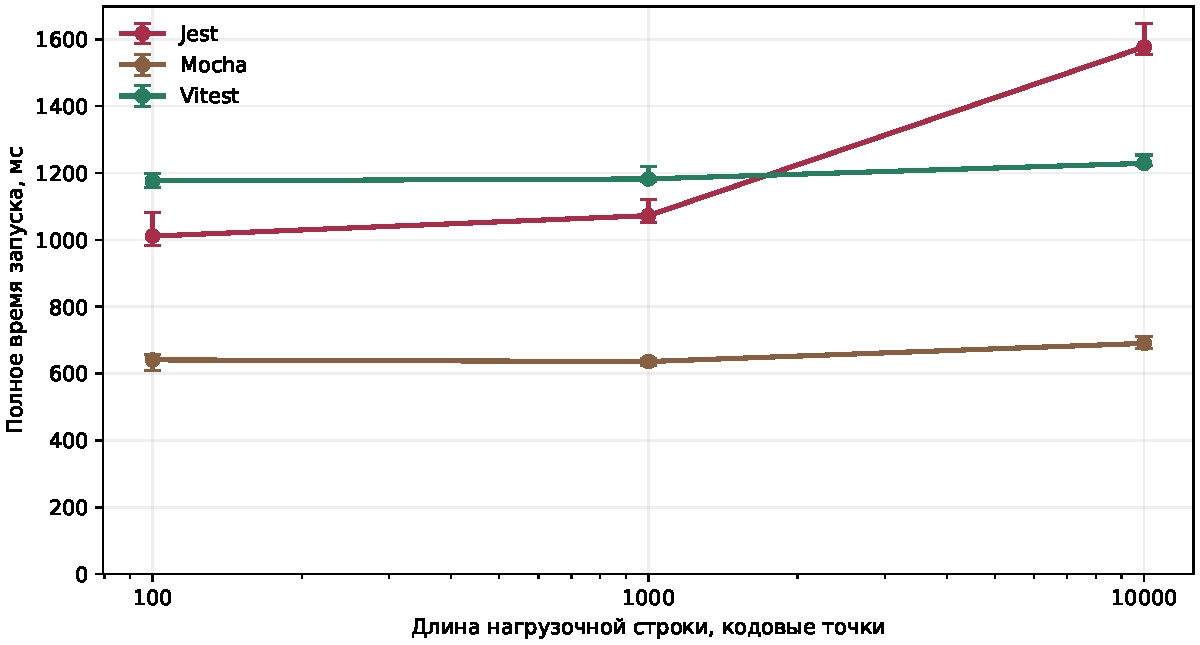
\includegraphics[width=.94\linewidth]{report/time.pdf}\caption{Полное время запуска. Точки -- медианы, отрезки -- первый и третий квартили.}\end{figure}

\begin{figure}[H]\centering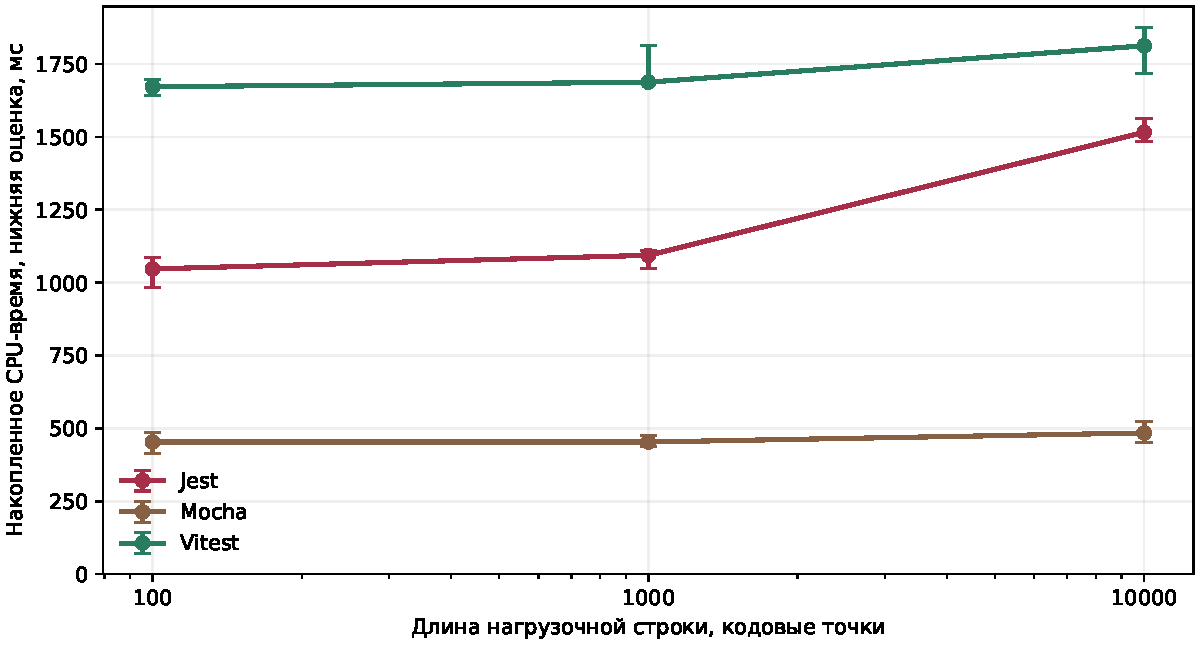
\includegraphics[width=.94\linewidth]{report/cpu.pdf}\caption{Накопленное CPU-время, нижняя оценка. Точки -- медианы, отрезки -- первый и третий квартили.}\end{figure}

\begin{figure}[H]\centering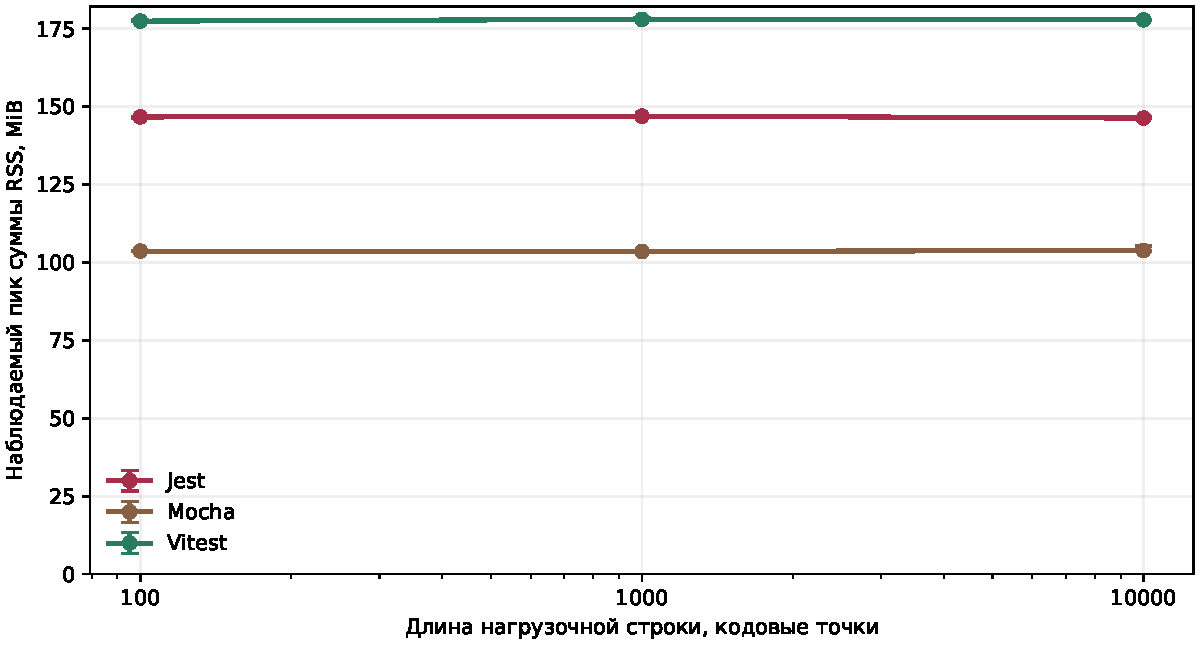
\includegraphics[width=.94\linewidth]{report/memory.pdf}\caption{Наблюдаемый пик суммы RSS. Точки -- медианы, отрезки -- первый и третий квартили.}\end{figure}

\begin{table}[H]\centering\small
\caption{Средняя CPU-загрузка в единицах одного логического процессора}
\begin{tabular}{rlrrr}\toprule
Длина & Раннер & Медиана, \% & $Q_1$ & $Q_3$\\\midrule
100 & Jest & 105.5 & 103.6 & 116.6\\
100 & Mocha & 88.5 & 84.2 & 101.1\\
100 & Vitest & 108.3 & 101.0 & 109.8\\
1000 & Jest & 110.7 & 105.3 & 115.4\\
1000 & Mocha & 90.9 & 87.9 & 95.6\\
1000 & Vitest & 104.4 & 100.3 & 108.1\\
10000 & Jest & 112.9 & 100.0 & 114.4\\
10000 & Mocha & 96.4 & 90.0 & 100.2\\
10000 & Vitest & 105.8 & 105.1 & 109.6\\
\bottomrule\end{tabular}\end{table}

В каждом запуске пройдены 99 тестов. Минимальное число отсчётов равно 41; максимальный интервал между обходами -- 30.6 мс. Обнаружено от 9 до 14 процессов на запуск. Различие числа обнаруженных процессов также может отражать пропуск коротких процессов при опросе.

\section{Обсуждение и ограничения}
Полное время включает постоянные и переменные составляющие. Условная модель
\[
 T_f(N,q)=A_f+B_f(N,q)+\varepsilon
\]
помогает интерпретировать результаты: $A_f$ включает создание процесса и инфраструктуру, $B_f$ -- работу с входом, а $\varepsilon$ -- изменчивость среды. По трём точкам нельзя надёжно оценить универсальную функцию затрат. Если время почти не изменилось при росте небольшого входа, это согласуется с существенной постоянной составляющей, но само по себе не определяет её точный размер.

Низкая средняя CPU-загрузка не обязательно означает меньшее процессорное время. Процесс может долго ожидать файловую систему и иметь малую долю CPU при большом времени ответа. Поэтому $\widehat C$ и $\widehat U$ показаны раздельно. При сравнении ресурсов приоритет имеет накопленное время, а процент помогает объяснить соотношение работы и ожидания.

Один worker Vitest не означает один поток операционной системы. Node.js и вспомогательные компоненты могут использовать собственные потоки; часть служб может существовать как дочерний процесс. Ограничивается параллелизм тестовых задач, а не всё внутреннее устройство среды. Сравнение не пытается сделать реализации раннеров идентичными: различия их инфраструктуры входят в предмет исследования.

Наблюдатель с дискретным опросом не гарантирует фиксацию короткого пика памяти. Отсчёты RSS разных процессов также не являются строго одновременными. Записанный максимум характеризует используемый метод измерения. Для точного учёта завершённых процессов потребовались бы механизмы ОС, например специализированная трассировка и учёт дерева задач, которые выходят за рамки компактного кроссплатформенного стенда.

Наконец, установка и прогрев могут менять состояние кэшей. Измерения выполняются на рабочей Windows-машине, а не на выделенном лабораторном сервере. В отчёте не заявлено, что все фоновые процессы были отключены. Повторный запуск способен дать другие абсолютные величины. Сохранённые версии и входы обеспечивают повторяемую процедуру, но не обещают побитовое совпадение временных показателей.

\section{Инструкция по установке и запуску}
Для программы требуются Node.js версии не ниже 22 с npm и Python версии не ниже 3.10. В данной апробации использованы конкретные версии, указанные в разделе результатов. Команды выполняются в каталоге \code{benchmark_app}. Интернет нужен при первой установке пакетов; измеряемые тесты после установки сетевых обращений не требуют.

\begin{lstlisting}
cd benchmark_app
npm ci
python -m venv .venv
.venv\Scripts\python.exe -m pip install -r requirements.txt
npm run verify
npm test
npm run demo
npm start -- --text "abba"
npm start -- --file data/input-example.json
npm run test:jest
npm run test:mocha
npm run test:vitest
\end{lstlisting}

Команды выше рассчитаны на Windows PowerShell. Активация окружения не обязательна: можно непосредственно вызывать его Python. В Linux и macOS вместо \code{.venv\Scripts\python.exe} используют \code{.venv/bin/python}. Программа JavaScript не требует отдельной компиляции. Команда \code{npm ci} устанавливает версии из lock-файла и пригодна для повторяемого code review.

Заготовленные входы включены в проект. Для пересоздания или изменения размера:
\begin{lstlisting}
.venv\Scripts\python.exe generate.py
.venv\Scripts\python.exe generate.py --sizes 200 2000 --cases 12
node src/demo.js data/author-palindromes.csv
\end{lstlisting}
Увеличение \code{--cases} повышает число записей, а \code{--sizes} -- длину каждой строки. После изменения нужно заново измерить производительность; старые результаты не описывают новые файлы.

Короткая проверка измерителя:
\begin{lstlisting}
.venv\Scripts\python.exe benchmark.py --input data/size-100.json --runs 2 --output reports/smoke
\end{lstlisting}
Основная серия:
\begin{lstlisting}
.venv\Scripts\python.exe benchmark.py --runs 7 --repeats 10 --output reports/new-json
\end{lstlisting}
Эквивалентная серия CSV:
\begin{lstlisting}
.venv\Scripts\python.exe benchmark.py --input data/size-1000.csv --runs 7 --output reports/new-csv
\end{lstlisting}

Если Node.js не находится в PATH, путь к исполняемому файлу передаётся через \code{--node}. Параметр \code{--timeout} задаёт предел в секундах. \code{--interval-ms} задаёт паузу опроса; изменение этого параметра требует новой серии и должно отражаться в интерпретации результатов. Запись производится в каталог \code{--output}, поэтому для сохранения прошлой серии выбирают новое имя.

Полная автоматическая приёмка запускается командой \code{.venv\Scripts\python.exe validate.py}. Она проверяет все три фреймворка, включая намеренно неверное ожидание. Сохранённые результаты новой апробации находятся в \code{reports/2026-09-16-json} и \code{reports/2026-09-16-csv}. Существующая серия не перезаписывается: при повторе следует выбрать новое имя каталога.

Для сборки документов нужны XeLaTeX и Biber из TeX Live или MiKTeX, пакеты Beamer, biblatex, algorithm и algpseudocode, а также шрифты Times New Roman, Arial и Consolas. Из корня проекта:
\begin{lstlisting}
xelatex -interaction=nonstopmode -halt-on-error My_thesis.tex
biber My_thesis
xelatex -interaction=nonstopmode -halt-on-error My_thesis.tex
xelatex -interaction=nonstopmode -halt-on-error My_thesis.tex
xelatex -interaction=nonstopmode -halt-on-error Presentation.tex
biber Presentation
xelatex -interaction=nonstopmode -halt-on-error Presentation.tex
xelatex -interaction=nonstopmode -halt-on-error Presentation.tex
\end{lstlisting}
Готовые PDF приложены, поэтому установка LaTeX не нужна для чтения и демонстрации. Для смены персональных данных редактируются титульные блоки двух исходников. При пересчёте экспериментальных результатов сначала обновляются автоматически генерируемые таблицы и диаграммы согласно README.

\section{Заключение}
По принятому правилу для исследуемого приложения выбран Mocha. Он получил 9 первых мест из девяти сравнений. При длине нагрузочной строки 10000 его медианы составили: 601.0 мс полного времени, 484.4 мс CPU-времени и 101.1 MiB наблюдаемого пика RSS. Выбор относится к полному набору из 99 тестов на данной машине; он не устанавливает универсального победителя для всех проектов.


Разработан компактный стенд сравнения Jest, Mocha и Vitest на общей алгоритмической нагрузке. Он импортирует файлы переменного размера в JSON и CSV, проверяет результат по эталону, выполняет одинаковые утверждения в трёх раннерах и сохраняет данные для воспроизведения эксперимента.

Содержательная проверка предшествует измерению скорости. Независимый перебор коротких строк, специальные случаи, метаморфное свойство и негативные входы проверяют разные классы ошибок. Пошаговый пример показывает связь между радиусами Манакера, найденной подстрокой и количеством палиндромных вхождений.

Сравнение учитывает полное время запуска, накопленное CPU-время и наблюдаемую память дерева процессов. Определения метрик позволяют не смешивать CPU-проценты с процессорным временем, а RSS -- с размером JavaScript-кучи. Ограничения дискретного опроса явно включены в методику и трактовку результатов.

Практический результат состоит в проверяемой процедуре выбора для заданной конфигурации. Полученные числа применимы к одному пакетному тесту чистой функции и указанной машине. Следующее развитие исследования -- несколько тестовых файлов, режим наблюдения, покрытие и прикладной набор проекта. Эти сценарии требуют отдельных серий, а не распространения текущего ранжирования без измерений.
\label{body-end}

